\part{Entwicklerhandbuch}

\chapter{Übersicht}
\section{Technologien und Werkzeuge}
Um die Anforderungen an das Software-Projekt bestmöglich zu erfüllen werden verschiedene Web-Technologien und -Werkzeuge zur Umsetzung des Projektes verwendet. Im folgenden wird erläutert, an welcher Stelle des Projektes diese eingesetzt werden und warum.

\paragraph{Javascript}
Die Skriptsprache \textit{Javascript} wird im vorliegenden Projekt als Programmiersprache verwendet.
Der aktuelle \textbf{ECMA-262}\footnote{\url{http://www.ecma-international.org/publications/standards/Ecma-262.htm}} Standard, welcher im Allgemeinen als \textit{ECMAScript 6} bezeichnet wird, ermöglichte hierbei eine objektorientierte Implementierung.

\paragraph{node.js}
Um die Ausführung von Javascript-Code außerhalb eines Browsers zu ermöglichen wird die Laufzeitumgebung \textit{node.js} verwendet.

\paragraph{React.js}
Durch die Nutzung des Javascript-Frameworks \textit{React.js} ist es möglich die Benutzerschnittstelle mit einem geringstmöglichen Aufwand zu implementieren und besonders effizient zu rendern.
Es wird hierbei der spezielle React-Syntax \textit{JSX} verwendet und mit sogenannten \textit{React-Komponenten} gearbeitet.
Diese Komponenten stellen dem Framework einen minimalen Satz an UI-relevanten Informationen bereit, welches dieses aufbereitet und somit in der Lage ist bei Änderungen ausschließlich jene Bereich erneuern, deren Daten sich tatsächlich verändert haben.

\paragraph{npm}
Um die Erfüllung von Abhängigkeiten im Laufe der Implementierung elegant und automatisiert zu gewährleisten wird die Javascript-Paketverwaltung \textit{npm} genutzt.
Diese wird über die Datei \texttt{package.json} im Root-Verzeichnis der Anwendung konfiguriert.

\paragraph{bower}
Während \textit{npm} vorrangig Backend-relevante Pakete verwaltet, ist die Paketverwaltung \textit{bower} auf Frontend-spezifische spezialisiert.
So wird bower beispielsweise verwendet um Pakete wie \textit{bootstrap} oder \textit{React.js} einzubinden.
Die Konfiguration findet hier ähnlich zu \textit{npm} über eine Kon"-fi"-gu"-ra"-tionsdatei (\texttt{bower.json}) statt.

\paragraph{grunt}
Bei der Implementierung der Anwendungen wird \textit{ECMAScript 6}, sowie \textit{LESS} zur Beschreibung der Styles benutzt.
Selbst moderne Browser unterstützen dieses Technologien jedoch nur bedingt, weshalb verschiedene sogenannte Transpiler notwendig sind.
Diese und weitere Aufgaben werden mit Hilfe des \textit{grunt}-Frameworks verwaltet und automatisiert durchgeführt.
Die Datei \texttt{Gruntfile.js} enthält hierbei die Konfiguration der Tools.

\paragraph{karma \& jasmine}
Neben manuellen Software-Tests wurden im Rahmen des Projektes ebenfalls automatisierte Testverfahren entworfen und angewendet.
Eine Kombination der Frameworks \textit{karma} und \textit{jasmine} bilden hierzu die Grundlage.


\section{Systemvoraussetzungen}
Neben einem beliebigem Texteditor benötigt man zur Weiterentwicklung der Anwendung zunächst eine \textit{node.js}-Kompatible Laufzeitumgebung. Dieses kann z.B. unter \url{https://iojs.org/} für verschiedene Plattformen bezogen werden.

\paragraph{}
Nach der Installation von \textit{node.js} können alle weiteren Pakete und Werkzeuge mit Hilfe der Paketverwaltung \textit{npm} nachgeladen werden.
Diese ist Teil der \textit{node.js}-Installation. Um diese zu tun sind die folgende Befehle in einer Kommandozeile einzugeben:
\begin{lstlisting}
	npm install -g grunt
	npm install -g bower
	npm install
	bower install
\end{lstlisting}

Nach der Installation dieser Pakete sind alle Systemvoraussetzungen für Weiterentwicklung dieser Anwendung erfüllt.

\section{Build-Prozess}
Wie bereits mehrfach erwähnt war die große Kompatibilität zu verschiedenen Plattformen ein Grund für die Entscheidung, das Projekt mit Web-Tech"-no"-lo"-gien umzusetzen.
Als \textit{Build-Prozess} wird in diesem Kontext die Routine bezeichnet, die aus dem Quellcode des Projektes die Pakete erzeugt, welche an Kunden und Benutzer ausgeliefert werden.

\paragraph{}
Der \textit{Build-Prozess} wurde im vorliegenden Projekt mit Hilfe des \textit{grunt}-Frame"-works automatisiert und soll im folgenden beschrieben werden.
Diese Beschreibung eignet sich zusätzlich als Einführung in die Arbeitsweise des \glqq Task-Runners \grqq \textit{grunt}. Dargestellte Listings sind der \textit{grunt}-Kon"-fi"-gurations"-datei \\\texttt{Gruntfile.js} entnommen.

\begin{lstlisting}[language=JavaScript,label=JS:grunt_build,caption=grunt build-Task]
grunt.registerTask('build', function (target) {
	grunt.task.run([
		'dist',
		'nodewebkit',
	]);
});
\end{lstlisting}

Zeile 1 im Listing \ref{JS:grunt_build} zeigt die \glqq Anmeldung\grqq des Tasks im Framework.
Dies hat zur Folge das der beschriebene Task im Wurzelverzeichnis der Anwendung durch Eingabe des folgenden Befehls in einer Kommandozeile \texttt{grunt serve} ausgeführt werden kann.
Dieser Task bündelt nun die Ausführung von \texttt{dist} und \texttt{nodewebkit}.

\newpage
\begin{lstlisting}[language=JavaScript,label=JS:grunt_dist,caption=grunt dist-Task]
grunt.registerTask('dist', function (target) {
	grunt.task.run([
		'clean:dist',
		'useminPrepare',
		'concurrent:dist',
		'postcss',
		'concat',
		'cssmin',
		'uglify',
		'copy:dist',
		'filerev',
		'usemin',
		'htmlmin',
	]);
});
\end{lstlisting}

\paragraph{}
Listing \ref{JS:grunt_dist} zeigt den Inhalt des \textit{dist}-Tasks.
Die einzelnen Punkte entsprechen wiederum verschiedenen Unteraufgaben, welche in Tabelle \ref{dist_table} näher beschrieben sind.

\paragraph{}
Diese Aufgaben dienen alle der Vorbereitung des Quellcodes um im Anschluss mittels \texttt{nodewebkit} die fertigen Anwendungen zu erstellen.
Listing \ref{JS:grunt_webkit_config} zeigt die Konfiguration der entsprechenden Aufgaben.
Neben Quell- und Zielordner sind hier die jeweiligen Zielarchitekturen eingetragen.

\begin{tabularx}{0.92\textwidth}{lX}
	\textit{clean:dist} & bereinigt temporäre und build-Ordner\\ \hline
	\textit{useminPrepare} & TODO\\ \hline
	\textit{concurrent:dist} & Konfiguriert verschiedene Unteraufgaben um Nebenläufigkeit im Build-Prozess zu erzeugen\\ \hline
	\textit{postcss} & TODO\\ \hline
	\textit{concat} & TODO\\ \hline
	\textit{cssmin} & Verringert die Größe der CSS-Dateien\\ \hline
	\textit{uglify} & Verringert die Größe der Javascript-Dateien\\ \hline
	\textit{copy:dist} & Kopiert alle notwendigen Dateien in die jeweiligen Veröffentlichungs-Unterordner\\ \hline
	\textit{filerev} & Ändert Dateinamen um Probleme mit dem Cache des Browser zu vermeiden\\ \hline
	\textit{usemin} &  TODO\\ \hline
	\textit{htmlmin} & Verringert die Größe der HTML-Dateien\\ \hline
\end{tabularx}
\label{dist_table}
\vspace*{1cm}

\begin{lstlisting}[language=JavaScript,label=JS:grunt_webkit_config,caption=grunt nodewebkit-Konfiguration]
nodewebkit: {
	options: {
		platforms: [
			'win32',
			'win64',
			'linux32',
			'linux64',
			'osx64',
		],
		buildDir: 'builds',
	},
	src: ['dist/**/*'],
},
\end{lstlisting}

\paragraph{}
Nach Abschluss dieses Tasks befinden sich die Versionen zur Veröffentlichung in Unterordnern \texttt{ win32, win64, linux32, linux64} und\texttt{ osx64 }des Ordners \texttt{ dist } im Wurzelverzeichnis der Anwendung.

\chapter{Software-Entwurf}
\section{Grobentwurf}
Eine Prämisse des Projektes war stets den Fahrstuhl inklusive Steuerung mög"-lichst realitätsnah zu simulieren. Daher wurde die Anwendung von Beginn an in Teilsysteme untergliedert.

\paragraph{Komponentenstrukt}
Dies zeichnet sich insbesondere in der Struktur der Anwendung aus, welche aus mehrere Komponenten besteht, die wiederum in der Realität existierende Teilsysteme eines Fahrstuhlsystems abbilden.
So unterteilt sich das Gesamtsystem \textbf{Fahrstuhlsimulation} zunächst in die Teilsysteme \textbf{Fahrstuhlsteuerung} und \textbf{Visualisierung}, welche weiterhin verschiedene Komponenten beinhalten.

\paragraph{}
Im Entwurf der \textbf{Fahrstuhlsteuerung} sind dementsprechend \textit{Steuerung}, \textit{Sensoren} und \textit{Schnittstellen zur Passagierinteraktion} in voneinander unabhängige Komponenten gekapselt, welche sich im Feinentwurf auch als Klassen des Software-Systems wiederfinden.

\paragraph{}
Zu den Sensoren der Fahrstuhlsimulation gehören \textit{Etagen-}, \textit{Tür-}, und \textit{Gewichtssensoren}.
Deren Kommunikation mit der Steuerung erfolgt ebenfalls über definierte Schnittstellen, wobei zusätzlich zu unterscheiden ist, ob es sich um aktive oder Passive Sensoren handelt.\todo{Welche Sensoren sind aktiv, welche Passiv?}

\paragraph{MVC-Paradigma}
Auf einer hohen Abstraktionsebene kann das System so auch unter dem MVC-Modell\footnote{Abk. für Model-View-Controler-Modell} betrachtet werden.
Die Intention besteht darin die Fahrstuhlsteuerung als Modell zu charakterisieren und die Kommunikation mit der Benutzerschnittstelle, der View, über einen Controller zu etablieren.
Somit Kommunizieren die verschiedenen Teilsysteme ausschließlich über definierte Schnittstellen und die Paradigmen Modularität und Wiederverwendbarkeit sind inhärent erfüllt.

\paragraph{Steuerungs-Algorithmus}
Neben der Struktur der Anwendung ist ebenfalls ein aus der Realität bekannter Algorithmus zur Steuerung des Fahrstuhls adaptiert worden, der sogenannte \textit{Fahrstuhl-Algorithmus mit Sammelsteuerung}\cite{wiki_elev}.
Dieser bedient zunächst Fahrtwünsche und -Rufe auf der aktuellen Fahrtrichtung und kehrt diese im Anschluss um.

\paragraph{}
Die Fahrstuhlsteuerung muss nun beim Erreichen einer Etage unter anderem zwei Fragen beantworten:

\begin{enumerate}
	\item Existiert ein Fahrtwunsch /-Ruf auf dieser Etage und muss dementsprechend angehalten werden?
	\item Existieren Fahrtwünsche /-Rufe ober- oder unterhalb der aktuellen Etage, beziehungsweise muss die Fahrtrichtung beibehalten oder umgekehrt werden?
\end{enumerate}

\paragraph{}
Frage 2. ist in dem Fall die interessantere.
Ein naiver Ansatz könnte folgendermaßen außen:\\ \\ Ein System besitzt $N$ Etagen, die Kabine befindet sich aktuell in Etage $M$ und fährt in Richtung $X$.
Um zu entscheiden ob die Fahrt in der aktuellen Fahrtrichtung fortgesetzt wird durchsucht die Steuerung die Datenstruktur der Etagen linear im Bereich $(M,N]$ für $X>0$ (aufwärts) oder im Bereich $[0,M)$ für $X<0$ (abwärts).\\\\
Dieser Algorithmus wäre jedoch abhängig von der Menge der Etagen und besäße damit die Komplexität $\mathcal{O}(n)$.

\paragraph{}
Beim Entwurf des Algorithmus der vorliegenden Anwendung war das Ziel diese Komplexität zu verringern.
Seine Funktion erklärt sich wie folgt:\\ \\ Grundlegendes Element des Algorithmus ist eine Datenstruktur, welche ausschließlich die \textbf{Summe} der Fahrtwünsche /-Rufe über- und unterhalb der aktuellen Position enthält.
Um nun über die Fahrtrichtung entscheiden zu können muss die Fahrstuhlsteuerung ausschließlich an definierten Stellen in dieser Datenstruktur überprüfen, ob Elemente größer 0 sind.
Die Komplexität dieser Abfrage über einer Datenstruktur fester Größe besitzt die Komplexität $\mathcal{O}(1)$, was einer Reduktion entspricht.
Zu beachten ist dabei jedoch, dass die genannte Datenstruktur zu jedem Zeitpunkt aktuell gehalten werden muss. Dies ist jedoch ein implementierungsspezifisches Problem, dessen Lösung in der Sektion \textit{\nameref{imp_model}} im Kapitel \textbf{\nameref{imp}} beschrieben wird.

\section{Feinentwurf}

\paragraph{React}
Wie bereits erwähnt wurde erleichtert das React Framework die Entwicklung performanter Webanwendungen.
Bei der bisher im Web üblichen Herangehensweise wurde in der Regel das HTML der Website Serverseitig gerendert.
Trat eine gewisse Änderung in dem Clientseitigen Model auf, z.B. weil dem Client vom Server neue Daten zugesendet wurden, so wurde \textit{explizit} der jeweilige Bereich der Seite, welcher diese Daten darstellte, erneuert.
Die einzigen zwei Möglichkeiten um dies zu erreichen, sind hierbei natürlich nur die, die jeweiligen \textit{explizit} Attribute einer \textit{DOM-Node}, wie z.B. Farbe, oder den Text, der Bereiche zu ändern, oder aber den gesamten Bereich in neuem HTML zu rendern.
Wie man sich leicht Denken kann, führt Ersteres eventuell zu der Frage, welcher Teil des Codes für was Verwantwortlich ist, oder aber erschwert die Entwicklung durch eine Überzahl an nötigen Controllern.
Letzteres wiederum ist eine eventuell äußerst inperformante Lösung, da das rendern von ganzen Bereichen der Seite auch jene betrifft die sich möglicherweise gar nicht geändert haben. \\

Als zur Zeit noch äußerst moderne Lösung bietet sich hierfür das aufstrebende React Framework, welches seit seiner Veröffentlichung mit Worten wie \glqq Bahnbrechend\grqq und \glqq Revolutionär\grqq betitelt.
Hierbei schreibt der Entwickler sogenannte React-Komponenten.
Statt nun bei einem Render-Vorgang dem React Framework fertigen HTML Code zu liefern, den die jeweilige Komponente darstellen will, muss sie stattdessen eine ebenso hierarische Objektstruktur zurückgeben, welche \textit{repräsentativ} für den HTML Code steht.
Diese repräsentative Struktur ähnelt dem und simuliert den sogenannten \textit{Document Object Model} (DOM), weshalb man diese Struktur auch den \textit{Shadow DOM} nennt.
Bei jeder Änderung des Zustands einer Komponente wird hierbei nun die \textit{render}-Methode neu aufgerufen.
Ändert sich zwischen 2 Aufrufen der \textit{Shadow DOM}, so wird ein möglichst minimaler Satz an Modifikationen berechnet, welche nötig sind um den alten \textit{Shadow DOM} in den neuen zu transformieren.
Dieser Satz an Änderungen wird nun auf den tatsächlichen \textit{DOM} des Browsers angewendet. \\

Diese Vorgehensweise ist selbstverständlich nicht so performant wie eine optimale und explizite Verwaltung des HTML und des \textit{DOMs}, jedoch ist die Performanz für nahezu alle Einsatzgebiete bei weitem ausreichend.
Da die Komplexität bei größeren Projekten jedoch stark zunimmt und somit eine optimale und explizite Verwaltung exponentiell schwieriger wird, übersteigt die Performance einer Website die React verwendet meistens die einer ohne.
Zusätzlich eleminiert React die Frage gänzlich, wie und wo man Änderungen auf eine Website anwenden und verwalten kann und ermöglicht somit zusätzlich eine äußerst schnelle Entwicklung.

\paragraph{Publish/Subscribe Pattern}
In der Web-Entwicklung ist zur Zeit eine Komponentenorientierte Entwicklung gebräuchlich, bei denen die Komponenten untereinander nur lose gekoppelt sind.
Um dies zu erreichen wird in der Regel das \textit{Publish/Subscribe} (PubSub) Pattern verwendet, welches dem traditionellen \textit{Observer} Pattern sehr ähnlich ist.
Statt sich als Objekt beim Subjekt explizit registrieren zu müssen, existiert hier ein Datenkanal welcher sogenannte \textit{Events} an alle \textit{Subscriber} verteilt.
Jedem Objekt steht es frei sich als \textit{Subscriber} bei diesem Kanal für einen bestimmten \textit{Event}-Typen ein- und auszutragen.
Des Weiteren existiert exakt ein Objekt welches als \textit{Publisher} fungiert und \textit{Events} eines bestimmten Typs mit einer beliebigen Anzahl an Parametern an alle Subscriber versenden kann.
Die Idee ist es hierbei also die einzelnen Klassen und Komponenten noch loser zu koppeln und stärker voneinander zu trennen, indem man selbst die letzten Abhängigkeiten zwischen Objekt und Subjekt, wie sie im klassischen Observer Pattern existieren, eleminiert.
Besonders mit Programmiersprachen wie ECMAScript lässt sich dies sehr leicht erzielen, da Funktionen hier nur eine spezielle Form von Objekten und sogenannte \textit{Lambda}-Funktionen sind.
Sie können sowohl eine beliebige Anzahl an Parametern annehmen, als auch mit einer beliebigen Anzahl aufgerufen werden.
Es ist somit möglich und üblich das PubSub Pattern mit \textit{Lambda}-Funktionen zu nutzen, um sowohl eine dynamische Menge an \textit{Event}-Typen und \textit{Event}-Parametern verarbeiten zu können, als auch eine vollständige Entkopplung zwischen \textit{Publisher} und \textit{Subscriber} zu erreichen.

\paragraph{Klassendiagramm}
\begin{figure}[h!]
	\centering
	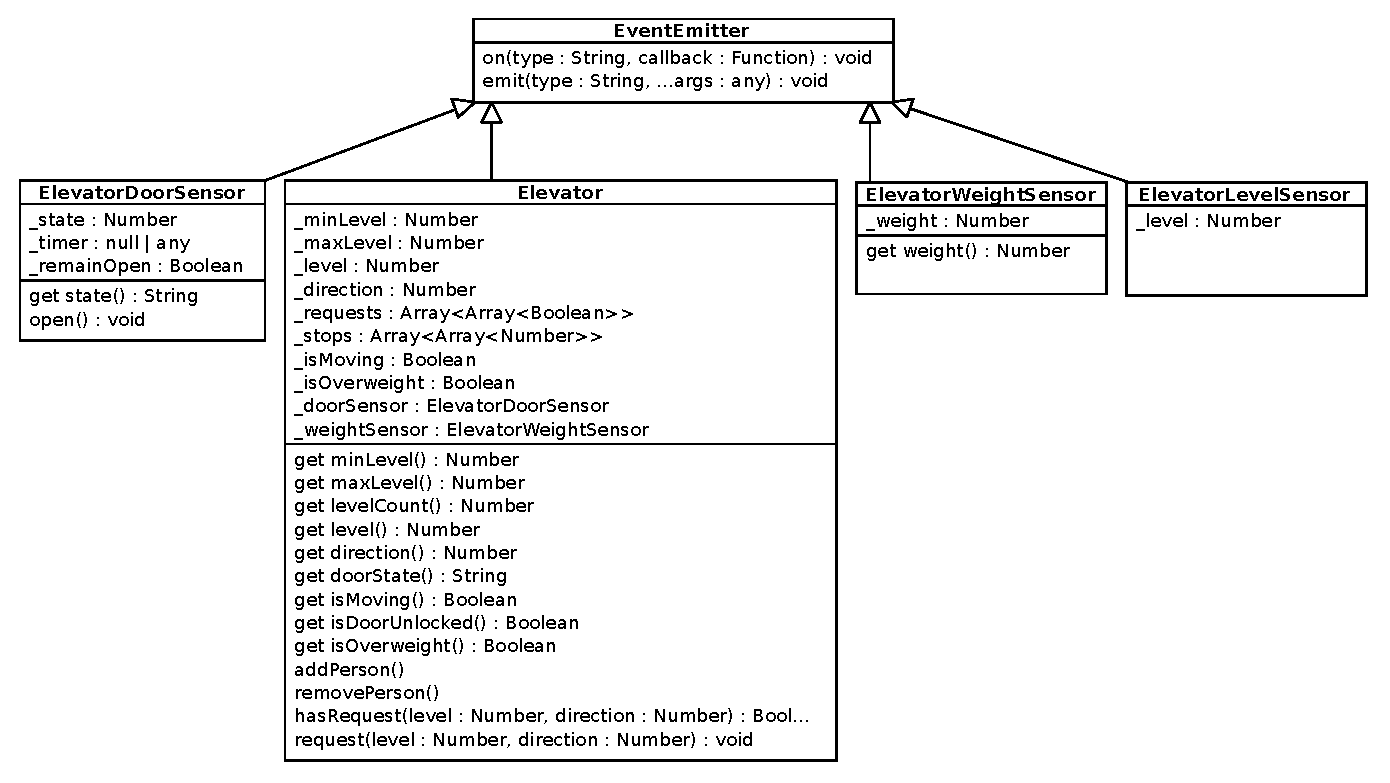
\includegraphics[width=0.9\textwidth]{images/klassendiagramm.eps}
	\caption{Übersicht der verwendeten Klassen der Hauptkomponente Fahrstuhlsteuerung}
	\label{klassdiagramm}
\end{figure}

\chapter{Implementierung}
\label{imp}

\section{Model}
\label{imp_model}
Als zentraler Kern des Model steht die Klasse \texttt{Elevator}.
Dieser steht in Verbindung mit seinen 3 Sensor-Klassen \texttt{ElevatorDoorSensor}, \texttt{ElevatorLevelSensor} und \texttt{ElevatorWeightSensor}.
Des Weiteren wird die \texttt{EventEmitter}-Klasse, welche das \textit{PubSub} Pattern implementiert und von \texttt{node.js}, bzw. von entsprechenden Shims für den Browser, zur Verfügung gestellt wird.
Wie im Entwurf bereits geplant wurde, sollen alle 4 \texttt{Elevator*} Klassen als möglichst eigenständige Komponenten existieren und erben deshalb alle von der \texttt{EventEmitter}-Klasse.
Während eine \texttt{Elevator}-Instanz also konstruiert wird, erstellt diese jeweils eine Instanz der 3 Sensor-Klassen und übergibt eine Referenz von sich selbst als Parameter.
Dadurch haben die Sensor-Klassen in ihren Konstruktoren Zeit sich beim \texttt{Elevator} als Subscriber für Events zu registrieren, die für sie relevant sind.
\textit{Keine} dieser Klassen hält jedoch eine explizite Referenz zum \texttt{Elevator} aufrecht, was die nötige Entkopplung für eine gute Komponentenarchitektur aufrecht erhält.
Der \texttt{Elevator} wiederum registriert sich selbst als Subscriber für die für ihn relevanten Events bei den Sensoren.
Der \texttt{Elevator} ist außerdem derjenige der eine Referenz zu den Instanzen der Sensorklassen aufrecht erhält --- man kann sagen, dass eine \texttt{Elevator}-Instanz \glqq Besitzer\grqq der Sensor-Instanzen ist.
Nahezu jegliche Kommunikation findet zwischen der Elevator-Instanz und einer Sensor-Instanz nun durch das \textit{PubSub} Pattern statt. \\

Die Elevator-Klasse, welche als \glqq Frontend\grqq des Models dient, stellt nun eine gewisse Zahl an öffentlichen Methoden zur Steuerung bereit, welche auch im Abschnitt \textit{\nameref{imp_api}} näher beleuchtet werden.
Die primäre Methode ist hierbei die \texttt{request}-Methode.
Wird versucht einen neuen Request hinzuzufügen, so wird dieser zunächst auf Validität geprüft.
Die überprüften Parameter sind die Etage zu der der Elevator fahren soll, als auch die ageforderte Richtung, welche als Integerwert übergeben muss.
Dieser Wert müssen wie auch an allen anderen Stellen die mit einer Fahrtrichtung arbeiten kleiner Null sein falls es ein Runter-, größer Null falls es ein Hoch- und gleich Null sein falls es ein Request vom Innentableau ist.
Ist er valide, so wird geprüft, ob sich der Elevator bereits auf der geforderten Etage befindet und still steht.
Sollte dies der Fall sein so wird nun die \texttt{open}-Methode des \texttt{ElevatorDoorSensor} aufgerufen.
Dies ist auch die zur Zeit einzige Verwendung eines direkten Methodenaufrufs im Model, da ansonten ein eigener Event-Typ einzig für diese eine Verwendung hätte hinzugefügt werden müssen und dies wäre nicht im Sinne des PubSub Patterns gewesen, welches eher auf eine 1:N-Verteilung abzielt.
Sollte dies alles jedoch nicht der Fall sein, so wird der Request dem Elevator hinzugefügt. \\

Die Requests werden hierbei in einem Array aus Boolean-Tripeln im Member \texttt{_requests} registriert.
Jedes Tripel in diesem Array steht hierbei repräsentativ für die noch ausstehenden Requests auf einer Etage entsprechend der Array-Position.
Hierbei, sowie in allen Weiteren Verwendungen von Tripeln in der Elevator-Klasse, ist das erste Element wahr falls auf der jeweiligen Etage ein Runter-Request aktiv ist.
Das zweite Element ist ebenfalls wahr falls ein Hoch-Request aktiv ist, sowie das dritte Element welches für einen Request aus dem Innentableau steht.
Des Weiteren existiert zusätzlich ein Tupel aus zwei gleichermaßen aufgebauten Integer-Tripeln, welches im Member \texttt{_stops} gespeichert wird.
Das erstere Tripel \textit{zählt} hierbei, wie bereits erklärt wurde, die jeweiligen Summen aller aktiven Requests unter und das Zweitere respektive alle über der aktuellen Elevator-Position. \\

Sollte sich der Fahrstuhl nun aktuell noch im Idle-Zustand befinden, so kann mittels der \texttt{_beginMoving}-Methode direkt in die entsprechende Richtung losgefahren werden.
Ist dies nicht der Fall und sind die Türen nicht verschlossen, so kommt der ElevatorDoorSensor ins Spiel. \\

Der ElevatorDoorSensor öffnet selbstverständlich die Türen sobald eine gewünschtes Ziel, bzw. ein Request, erreicht wird.
Dieses Ereignis wird vom Elevator mit dem \glqq stop\grqq-Event signalisiert und vom ElevatorDoorSensor aufgegriffen.
Dieser ruft nun seine \texttt{open}-Methode auf, welche eine interne State-Machine ins Rollen bringt, die die Zustände \textit{opening}, \textit{open}, \textit{shutting} und \textit{shut} abarbeitet.
Wie man bereits erkennen kann erfüllt der ElevatorDoorSensor trotz seines Namens nicht nur eine reine passive Sensor-, sondern auch eine Simulationsfunktion.
Bei einem Aufruf der \texttt{open}-Methode, sowie wenn ein State erreicht wurde, wird dessen Zustandsname als gleichnamiges Event verteilt und der nächste State mittels simplen Timern angesetzt, sofern nicht bereits der \textit{shut}-Zustand erreicht wurde, oder aber der \texttt{_remainOpen}-Member wahr ist.
Aufgrund der Implementierung des ElevatorDoorSensor als State-Machine, ist es in der Lage bei einem weiteren Aufruf der \texttt{open}-Methode die Timer zurückzusetzen, bzw. die Tür erneut zu öffnen, während sie aktuell offen ist, bzw. respektive während sie aktuell schließt. \\

Der Elevator greift hierbei nun das \textit{shut}-Event mit seiner \texttt{_onDoorShut}-Methode als Callback auf und versucht daraufhin gleichermaßen wie in der \texttt{request}-Methode loszufahren.
Da nun jedoch die Türen geschlossen sind so kann im Gegensatz zu vorher losgefahren werden. \\

Fährt der Elevator von einer Etage aus los so fährt so wird mit einem \textit{move}-Event die aktuelle Etage und die Fahrtrichtung signalisiert.
Hierfür wird nun der ElevatorLevelSensor relevant. \\

Der Elevator erstellt selbstverständlich bei der Konstruierung für jede Etage einen eigenen ElevatorLevelSensor.
Jeder dieser Instanzen registriert sich selbst bei dem Elevator für \textit{move}-Events.
Wird eines ausgelöst so erhält nun jeder Sensor in der Simulation eine Nachricht und jeder prüft ob es der Sensor wäre der der nächstgelegenen Etage in der Fahrtrichtung entspricht.
Dieser Sensor setzt nun einen Timer auf, welcher nach einer festen Zeit ein \textit{contact}-Event auslöst. \\

Der Elevator wiederum registriert sich bei der Konstruierung mit seiner \texttt{_onLevelContact}-Methode für die \textit{contact}-Events bei jedem ElevatorLevelSensor.
Wird eines ausgelöst signalisiert dies dem Elevator den Kontakt, bzw. die Ankunft, bei einer Etage.
Diese Ankunft macht der Elevator nun publik indem er zunächst ein \textit{change:level}-Event auslöst.
Sollte des Weiteren auf der nun angekommenen Etage ein Request vorliegen so wird außerdem ein \textit{stop}-Event ausgelöst, der Request aus \texttt{_requests} entfernt, sowie der entsprechende Eintrag in \texttt{_stops} dekrementiert.
Dieses Event wird unter anderem vom ElevatorDoorSensor aufgegriffen, welcher dadurch die Türen öffnet.
Die \texttt{_onLevelContact}-Methode implementiert hierbei außerdem das Kernstück des sogenannten Aufzug-Algorithmus.
Es wird also solange in die aktuelle Bewegungsrichtung weitergefahren bis keine Requests mehr in die Richtung vorliegen.
Ist dies der Fall so wird die Gegenrichtung geprüft und entsprechend die Richtung umgekehrt.
Sollte auch in der Gegenrichtung keine Requests vorliegen so wird ein \textit{idle}-Event ausgelöst.
\texttt{_stops} hilft hierbei enorm, da auf Iterationen durch das Requests-Array verzichtet werden kann.
Sollte der Fahrstuhl jedoch weiterfahren, so muss nun das nächste \textit{move}-Event ausgelöst werden.
Bevor dies geschiet wird jedoch sichergestellt, dass wenn der Fahrstuhl einen Request in die entgegengesetzte Richtung überspringt, die entsprechenden Summen in \texttt{_stops} angepasst werden, indem dessen gedachter Eintrag von der einen Seite des Fahrstuhls auf die anderen Seite übertragen wird. \\

Zuletzt existieren öffentliche APIs im Elevator um Personen hinzuzufügen, bzw. um sie zu entfernen.
Aufrufe dieser Methoden führen jeweils dazu, dass ein \textit{persons:add}-, bzw. respektive ein \textit{persons:remove}-Event ausgelöst wird.
Dieses Events werden vom ElevatorWeightSensor aufgegriffen, welcher sich bei seiner Konstruierung beim Elevator hierfür registriert, welche jeweils dazu führen, dass der ElevatorWeightSensor seinen Member \texttt{_weight} um den fixen Wert des Gewichts einer Person vergrößert, bzw. verringert.
Wird das maximale Gewicht überschritten, oder aber wieder unterschritten nachdem das maximale Gewicht bereits erreicht wurde, so wird ein \textit{change}-Event ausgelöst, welches als einzigen Parameter übermittelt, ob der ElevatorWeightSensor aktuell Überlast, oder Normallast meldet. \\

Dieses Event wird hierbei vom Elevator wiederum aufgriffen, welcher den Zustand zwischenspeichert und als Mediator das Ereignis als \textit{overweight:change}-Event weiterleitet.
Der ElevatorDoorSensor registriert sich beim Elevator nun außerdem in seinem Konstruktur für eben jenes Event, setzt seinen \texttt{_remainOpen}-Member entsprechend und ruft die \textt{open}-Methode auf.
Wie bereits erwähnt wurde sorgt nun ein Wahr-Wert im \texttt{_remainOpen}-Member dafür, dass ElevatorDoorSensor im \textit{open}-Zustand verbleibt.

\section{View/Controller}
\label{imp_vc}

\section{Benutzerschnittstelle}
Damit die aktiven Zustände hervorgehoben werden können, müssen sie eindeutig identifizierbar sein.
Dafür wurden die Elemente der Grafik gruppiert und mit IDs versehen, auf die mittels Javascript und dem \acrshort{DOM} zugegriffen werden kann.
Abbildung \ref{fig:ZD_id_view} stellt die Identifikatoren dar.
Bei der Benennung der IDs wurden folgende Konventionen angwendet:
\begin{itemize}
	\item präfix uml- für alle Bezeichner
	\item Worte durch Bindestriche getrennt
\end{itemize}

\begin{figure}[hbt]
	\centering
	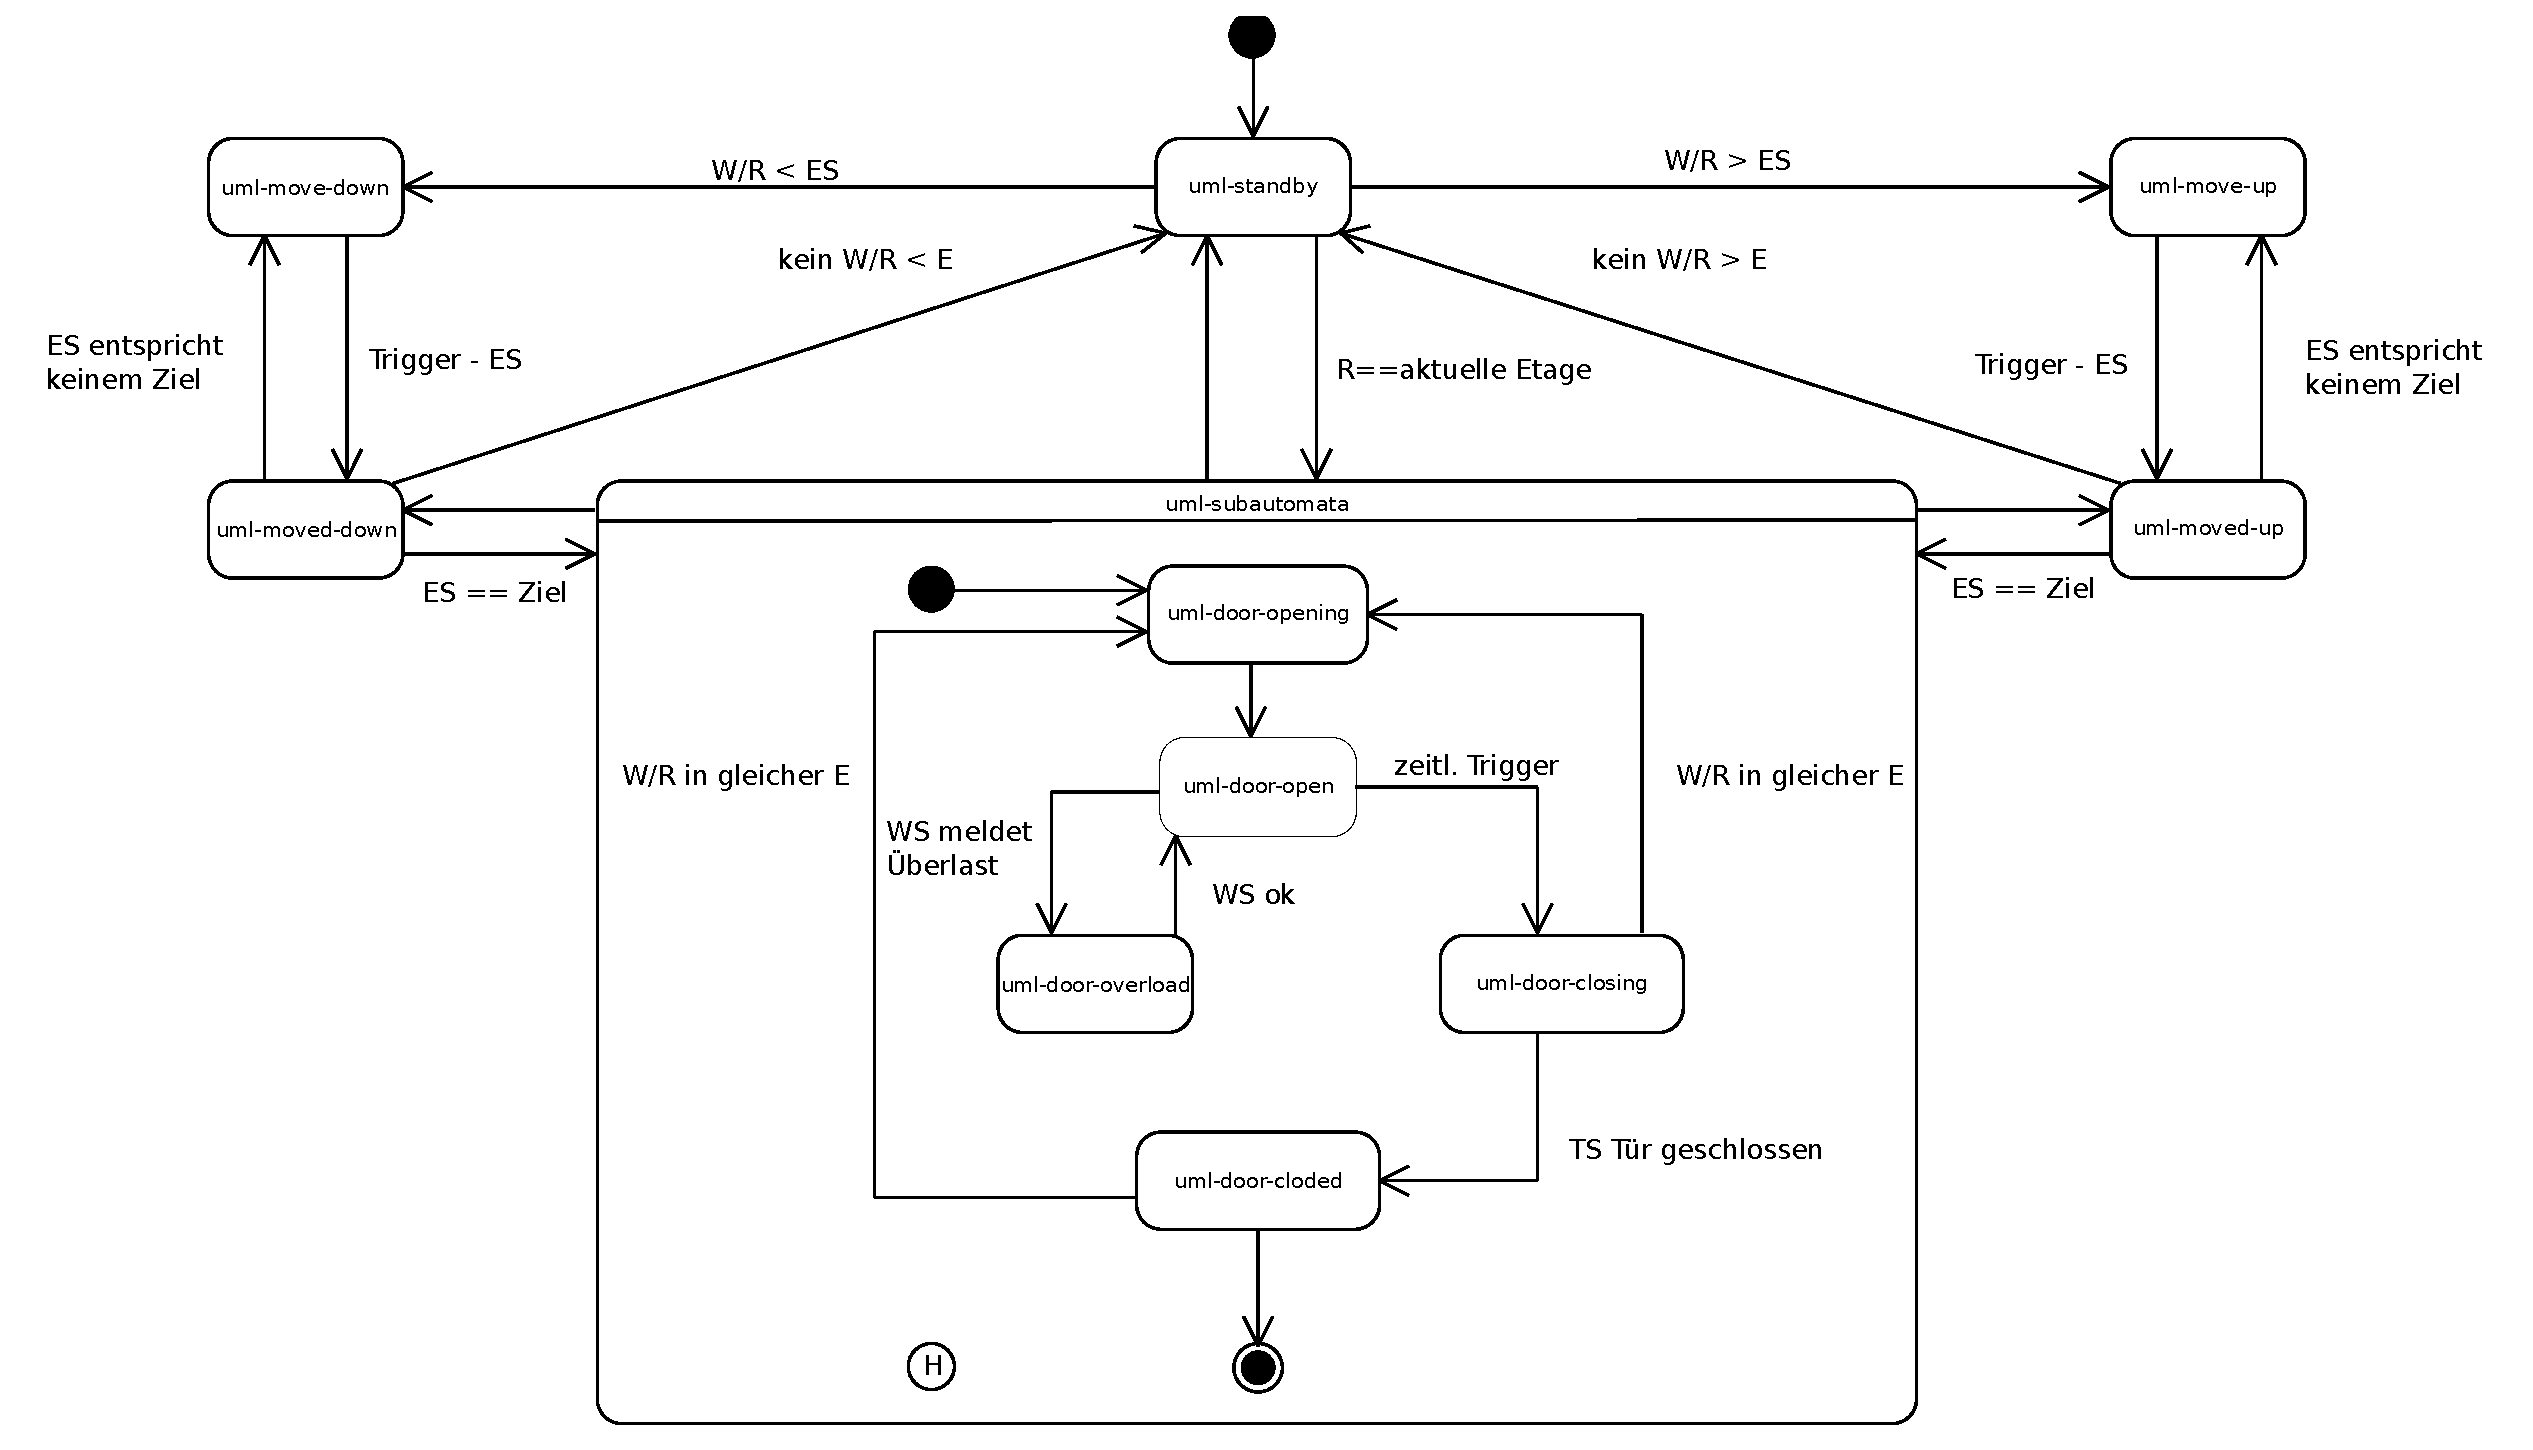
\includegraphics[width=\textwidth]{images/ZDv6_id_view.eps}
	\caption{IDs des Zustandsdiagrammes}%
	\label{fig:ZD_id_view}%
\end{figure}

\section{API}
\label{imp_api}

\section{Erweiterungen}
